\chapter{Wolterミラーの誤差応答シミュレーション}
\thispagestyle{empty}
\label{chap2}
\graphicspath{{chap2/figure/}}
\minitoc

\newpage
%%%%%%%%%%%%%%%%%%%%%%%%%%%%%%%%%%%%%%%%%%%%%%%%%%%%%%%%%%%%%%%%%%%%%%%%%%%%%


% ================================================== %
% section
% ================================================== %
\section{諸言}
\label{chap2_introduction}

Wolterミラーを光学系に組み込んで利用する際、大きく分けて2つの誤差によってその理想の集光・結像が損なわれる。
ひとつは設計曲面と実際に加工されたミラー表面の形状の誤差、もうひとつはミラー設置時の位置・姿勢の誤差である。
誤差応答、すなわちこれらの誤差が存在する際に集光点の様子がどのように変化するかを調べることで、Wolterミラーの利用時に求められる性能を発揮する上で許容される誤差の量が計算できる。
また、可視光光源を用いた位相回復法によってこれらの許容誤差範囲に収まっているかどうか判定することが可能であるかどうかを知る必要がある。
これらを踏まえ、本章では3段階に渡って誤差応答シミュレーションを行う。
まず、実際にWolterミラーが用いられるX線領域のうち2つの代表的な波長について、各種の誤差を入力した際の集光波面を算出し、許容できる誤差量を計算する。
続いて、ちょうど許容誤差の限界値ぶんの誤差がミラーに存在する場合に可視光を入射した際の位相分布を計算し、可視光による測定が可能であるかどうか、また可能であるならばどういった測定仕様を満たす必要があるかを計算する。
最後に、可視光計測において位相回復法から得られる波面誤差分布から各種誤差への分解を行うため、それぞれの誤差に対応する波面誤差分布をZernike多項式によって表現する。

\clearpage
% ================================================== %
% section
% ================================================== %
\newpage
\section{誤差の評価と許容される誤差}
\label{chap2_beam_evaluation_standard}

理想の集光波面との差異を定量的に評価するためには、具体的な評価軸が必要である。
そこで主に用いられるのが、Strehl比、HPD、FWHMの3つの特徴量である。

\subsection{Strehl比}
\label{chap2_strehl_ratio}
主に集光光学系の文脈において、理想の集光状態を「回折限界集光」と呼ぶ。
回折限界集光の状態にあるかどうかを判別する1つの指標として用いられるのが、Strehl比である。
Strehl比とは、実際の集光波面における最大値と回折限界時の集光波面における最大値の比として定義される。
つまり、振幅を$I(\mathbf{r})$として

\[
r_{\mathrm{Strehl}} = \frac{ \max{\sqrt{I(\mathbf{r})} } }{ \max{ \sqrt{I_{\mathrm{ideal}}( \mathbf{r} )} } }
\]

と定まる。
図\ref{fig:strehl_explanation}にその模式的なグラフを示す。
Strehl比を評価する基準として、Marechal基準\cite{BornWolf:1999:Book}が知られている。
Marechal基準では、Strehl比が0.8以上であるときその系は回折限界集光をしている、とする。
この0.8という値には体系的な根拠はなく、解析・実験における経験的な指標として扱われている。
本論文では、この慣例を踏襲し、0.8を閾値としてStrehl比を評価する。

\begin{figure}[h]
\centering
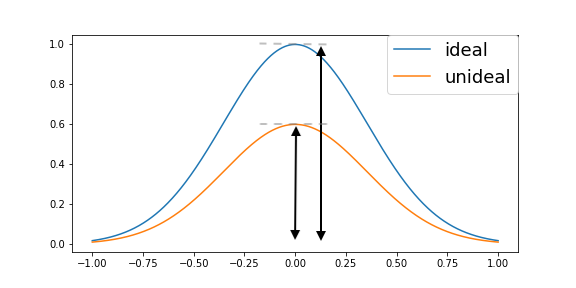
\includegraphics[width=10cm]{strehl.png}
\caption{Strehl比計算の模式図}
\label{fig:strehl_explanation}
\end{figure}

\subsection{HPD (Half Power Diameter)}
\label{chap2_hpd}

Strehl比による比較検討では「回折限界集光をしているか」に主眼を置いているが、天文用Wolterミラーのように達成すべき角度分解能が決まっている場合では、直接その分解能要求を満たしているかどうかを判定するのが実用的である。
分解能を決定するのは、焦点面におけるビームの集光サイズであり、これは大きく2つの定義によって議論される。
その一つが、Half Power Diameter(HPD)である。HPDの定義は「焦点面上の全強度の50\%の強度を含む円の直径」である。つまり、
\[
    \sum_{d\leq d_{\mathrm{HPD}}} \sqrt{ I(\mathbf{r}) } = \frac{1}{2} \sum \sqrt{ I(\mathbf{r}) }
\]
を満たすような直径$d_{\mathrm{HPD}}$として定義される。
図\ref{fig:hpd_explanation}にその例を示す。
この赤円の内側の強度総和値は、全体の強度総和値の半分になっている。

\begin{figure}[!ht]
\centering
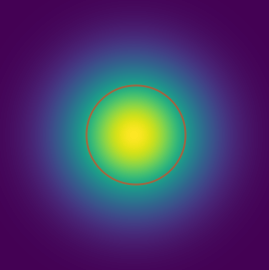
\includegraphics[width=6cm]{HPD.png}
\caption{HPDの例}
\label{fig:hpd_explanation}
\end{figure}

あるHPDを持つようなのふたつの結像点を分離できるような限界の配置が図\ref{fig:hpd_resolution_limit}のときであるとするならば、1秒角分解能という達成目標は図\ref{fig:hpd_arcsecond}が示すようなHPDで言い換えることができる。
つまり、ミラー上流端中心から半径を見込む角度がちょうど1秒角となるようなHPDが達成目標となる。
具体的には、ミラー上流端開口から焦点面までの距離2.1025 mに対してHPDは\SI{10.19}{\micro \metre}と計算される。
HPDを指標とした評価では、これを基準とする。

\begin{figure}[ht]
\centering
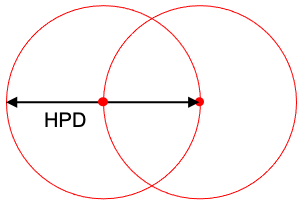
\includegraphics[width=6cm]{hpd_resolution_limit.png}
\caption{解像限界の図}
\label{fig:hpd_resolution_limit}
\end{figure}

\begin{figure}[ht]
\centering
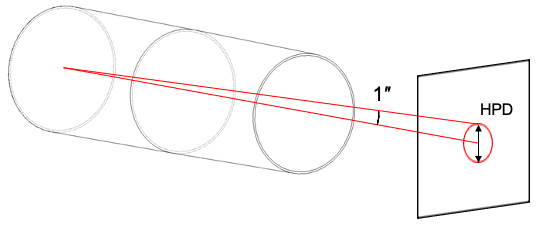
\includegraphics[width=12cm]{hpd_arcsecond.png}
\caption{HPDと結像分解能の関係}
\label{fig:hpd_arcsecond}
\end{figure}


\subsection{FWHM (Full Width Half Maximum)}
\label{chap2_fwhm}

HPDに並んでビーム集光サイズの評価として用いられるのが、FWHM(Full Width Half Maximum)である。
こちらは焦点面を集光点を通る直線によって切断したプロファイルに対して、「焦点面における最大値の半分の値を取る2点の距離」と定められる。
図\ref{fig:fwhm_explanation_profile}は1つのプロファイルに対するFWHMの例である。
切断する直線には任意性があるため、通常は図\ref{fig:fwhm_explanation}のように水平方向と鉛直方向の2方向に関して切断しこれを評価する。
\ref{chap2_ideal_focusing}節で具体的な計算例を示すが、結像性能の強いWolterミラーはメインピークに対して比較的大きいサブピークが細かく連なるような集光面強度分布を持つ。
そのため、強度はメインピークより外側に広がって存在しており、解像限界を決める上ではHPDの方が適していると言える。
FWHMはミラー開発の目標に対する評価ではなく、本研究中でのパラメータ設定の指標として用いることとする。

\begin{figure}[ht]
\centering
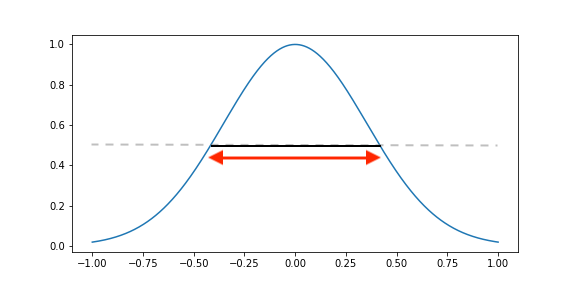
\includegraphics[width=8cm]{FWHM.png}
\caption{FWHMの例}
\label{fig:fwhm_explanation_profile}
\end{figure}

\begin{figure}[!ht]
\centering

\subfloat[horizontal]{
    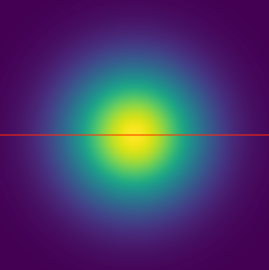
\includegraphics[width=5cm]{FWHM_horizontal.png}
    \label{fig:fwhm_explanation_horizontal}
}
\subfloat[vertical]{
    \centering
    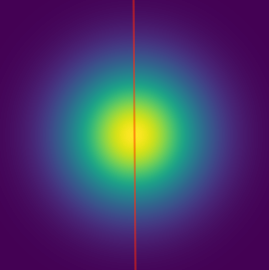
\includegraphics[width=5cm]{FWHM_vertical.png}
    \label{fig:fwhm_explanation_vertical}
}
\caption[]{切断の例 水平:\subref{fig:fwhm_explanation_horizontal}, 鉛直:\subref{fig:fwhm_explanation_vertical}}
\label{fig:fwhm_explanation}
\end{figure}


\clearpage
% ================================================== %
% section
% ================================================== %
\newpage

\section{Wolterミラーにおける光学波動場の伝播}
\label{chap2_wolter_diffraction_apporoximation}

シミュレーションおよび位相回復計算を行うにあたり、測定対象のWolterミラーの光学系において適用するべき波動場伝播の近似公式について検討する。
光学波動場の伝播に関しての詳細は付録において解説する。
まず、1章\ref{chap1_wolter_arrangement}節で示したパラメータについて、Fresnel回折近似の成立条件が成り立っているかどうかを確認する。
Fresnel回折近似が成り立つための条件は、近似で切り捨てる微小項が1 radより十分小さいときであり、これは式\ref{eqn:fresnel_approximation_condition}で表される。
ただし$z$は伝搬距離、$\lambda$は波長、$(x, y), (\xi, \eta)$は実空間および逆空間の座標を表す。

\begin{equation}
\label{eqn:fresnel_approximation_condition}
    \frac{\pi}{4\lambda} \max \left\{ (x-\xi)^2 + (y-\eta)^2 \right\}^2 / z^3 \ll 1
\end{equation}

焦点面を3章\ref{chap3_dynamic_range}節に示したCCDカメラのサイズとして取りこれを計算すると、(左辺)の値は1.645 radとなった。
これは十分小さいとは言えず、Fresnel回折近似を満たしているとは言えない。
しかし、Fresnel回折近似を満たしていない場合でも、計算を進めていく上でそれがほとんど影響を及ぼさない場合がある。
位相回復計算においては数万回の伝搬計算を行うため、1回のコストは最小限であることが好ましい。
そこで、厳密計算であるRayleigh-Sommerfeld回折積分とFresnel回折積分近似の集光面強度分布を比較し、実用上の問題が存在するかどうかを検討する。
まず、表\ref{tb:check_approximation_validity_1}に示すような適当な分割で回折積分を実行し、集光波面分布におけるメインピークのFWHMを調べる。

\begin{table}[!ht]
\begin{center}
  \begin{tabular}{|c|c|} \hline
    項目 & 値 \\ \hline
    波長 & 632.8 nm \\
    画素数 & $2048 \times 2048$ \\
    焦点面ピクセルサイズ & \SI{5.0}{\micro \metre} \\ \hline
  \end{tabular}
  \caption{Fresnel回折近似適用可能性の検討1}
  \label{tb:check_approximation_validity_1}
\end{center}
\end{table}

計算の結果、プロファイルは図\ref{fig:fwhm_approximation}のようになった。

\begin{figure}[ht]
\centering
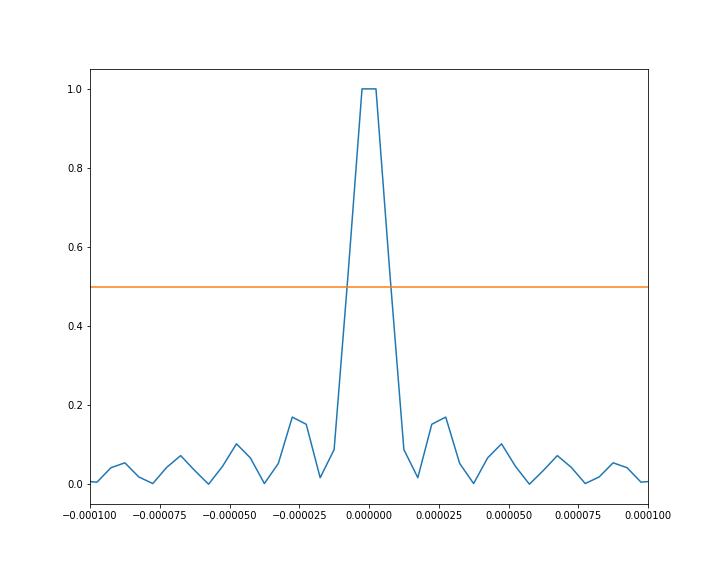
\includegraphics[width=8cm]{../../chap2/figure/fwhm_approximation.png}
\caption{回折積分計算による簡易的な計算で得られた焦点面強度プロファイル}
\label{fig:fwhm_approximation}
\end{figure}

ここから計算されるFWHMは4ピクセル分の\SI{20}{\micro \metre}であった。
これを踏まえ、メインピークを十分な分割数で観察できるよう焦点面ピクセルサイズが\SI{1}{\micro \metre}になるような表\ref{tb:check_approximation_validity_2}のパラメータで回折積分およびFresnel回折近似を用いた場合の集光面強度プロファイルを計算し、比較を行う。

\begin{table}[!ht]
\begin{center}
  \begin{tabular}{|c|c|} \hline
    項目 & 値 \\ \hline
    波長 & 632.8 nm \\
    画素数 & $4096 \times 4096$ \\
    焦点面ピクセルサイズ & \SI{1.0}{\micro \metre} \\ \hline
  \end{tabular}
  \caption{Fresnel回折近似適用可能性の検討2}
  \label{tb:check_approximation_validity_2}
\end{center}
\end{table}

計算の結果、プロファイルは図\ref{fig:diffraction_comparison}のようになった。
また、2つのプロファイルの差分を取って回折積分の最大値で規格化したグラフが図\ref{fig:diffraction_comparison_normalized_diff}である。

\begin{figure}[!ht]
\centering

\subfloat[プロファイルプロット]{
    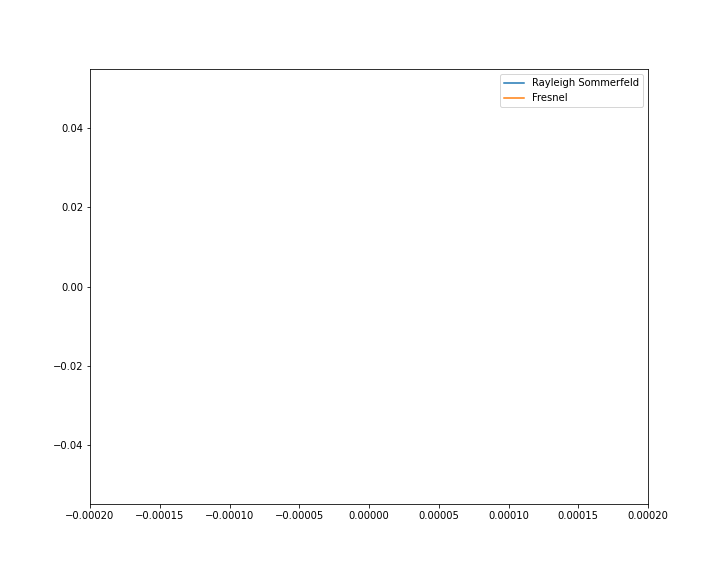
\includegraphics[width=6cm]{../../chap2/figure/diffraction_comparison_profile.png}
    \label{fig:diffraction_comparison_profile}
}
\subfloat[規格化されたプロファイル誤差]{
    \centering
    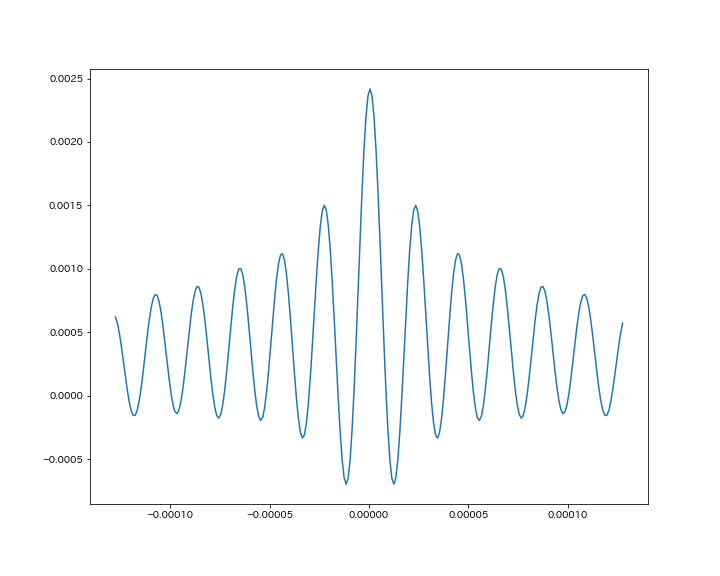
\includegraphics[width=6cm]{../../chap2/figure/diffraction_comparison_normalized_diff.png}
    \label{fig:diffraction_comparison_normalized_diff}
}

\caption[]{Rayleigh-Sommerfeld回折積分とFresnel回折積分のプロファイル比較}
\label{fig:diffraction_comparison}
\end{figure}

差分の絶対値の最大値は0.00242程度となった。
これは十分小さく、実際の計測で生じうるノイズと同程度以下であるため、シミュレーションでの検討および位相回復計算を行う上で致命的な問題をもたらさない。
ゆえに、以降の伝搬計算はFresnel回折近似を用いて行う。


\clearpage
% ================================================== %
% section
% ================================================== %
\newpage


\section{シミュレーションの方法}
\label{chap2_simulation_methodology}

この節では、シミュレーションの方法について述べる。
誤差応答シミュレーションは、図\ref{fig:simulation_schematic}に示すように、ミラー反射光が生成する下流端面における集光ビームの位相分布を求め、そこから焦点面に伝播するという流れに沿って行われる。
多数の条件に対して効率よくシミュレーションを行うため、下流端面上の波動場計算は幾何光学に基づいて行い、また下流端面から焦点面への伝播は\ref{chap2_wolter_diffraction_apporoximation}節に述べたようにFresnel回折近似を用いて計算する。
以下に具体的なシミュレーションの手順を示す。

\begin{enumerate}[\expandafter\maru 1]
  \item 放物面および双曲面について、ミラー表面の表現$f(x, y, z)=0$を理想形状の場合と誤差を考慮した場合それぞれについて与える。理想形状のミラーの場合、これは具体的に式\ref{eqn:parabola_surface_func}および式\ref{eqn:parabola_surface_func}のように与えられる。 \\
    \begin{eqnarray}
        f_p(x, y, z) &=& x^2 + y^2 - \left|4p(z-p-f2)\right| = 0 \label{eqn:parabola_surface_func} \\
        f_h(x, y, z) &=& \frac{\left(z - \frac{(f1 + f2)}{2}\right)^2}{a^2} - \frac{x^2 + y^2}{b^2} - 1 = 0 \label{eqn:hyperbola_surface_func}
    \end{eqnarray}
  \item 次に、図\ref{fig:simulation_raytrace}に示すように、ミラー下流端面を$N \times N$の小領域に分割し、ミラー形状から計算される定義域内の各点について幾何光学に基づいて以下のように光路長を計算することで、集光波面を求める。
    \begin{enumerate}[(1)]
      \item 下流端面上の点をPとする。
        誤差のない理想形状のミラーによって2回の反射の後Pに到達するような入射光線を求める。
        具体的には、焦点からPに向かう光線を双曲面、放物面の順に反射すれば、得られた光線が入射光線となる。
        反射の計算について、反射点は光線と\expandafter\maru 1 で与えた$f(x, y, z)=0$との交点として、また反射光の向きは反射の法則から$\mathbf{r} = \mathbf{i} + 2 (-\mathbf{i} \cdot \mathbf{n}) \mathbf{n}$として計算できる。
      \item 求めた入射光線を初期値として光線位置を$x, y$方向に動かして最適化し、誤差を入力したミラーにおける入射光線を求める。
        最適化計算はBroyden法で行う。
        入射光線の位置$(x, y)$を変数、2回反射後の下流端面における目標の点との位置誤差を目標値$\mathbf{E}$として、$\mathbf{E}=\mathbf{0}$を解けばよい。
        入射光線を$(x, y)$を通る$z$軸に平行な直線として与え、2回反射後の下流端面における目標の点との位置誤差を$\mathbf{0}$に近づけるようにこれを動かす。
      \item 求めた入射光線に対してミラー上流端面から下流端面に至るまでの距離$L$を計算し、点$P$での位相を$k L$(波動場を$\exp(i k L)$)として点$P$に関する計算を終了する。
    \end{enumerate}
  \item 次に、\expandafter\maru 2 で求めた下流端面上の各点$P$に対応する光路から、集光面の光軸方向位置の最適化を行う。
    図\ref{fig:simulation_focal_point_optimize}下流端面から集光点に向かう光線の$z=f$上の分布に対し、重心点と各点の距離の2乗和を$E$とする。
    $E$を最小化するように$f$を変化させることで、収束した$f$と重心点を$G(x_G, y_G)$から焦点位置が$F(x_G, y_G, f)$と定まる。
    初期値には理想の焦点距離$f_1$を与え、最適化は黄金探索によって行う。
  \item 最後に、下流端面から焦点面$z=f$に向かって$(x, y)=(x_G, y_G)$を光軸としてFresnel近似を利用した伝播計算を行う。
\end{enumerate}

\begin{figure}[h]
\centering
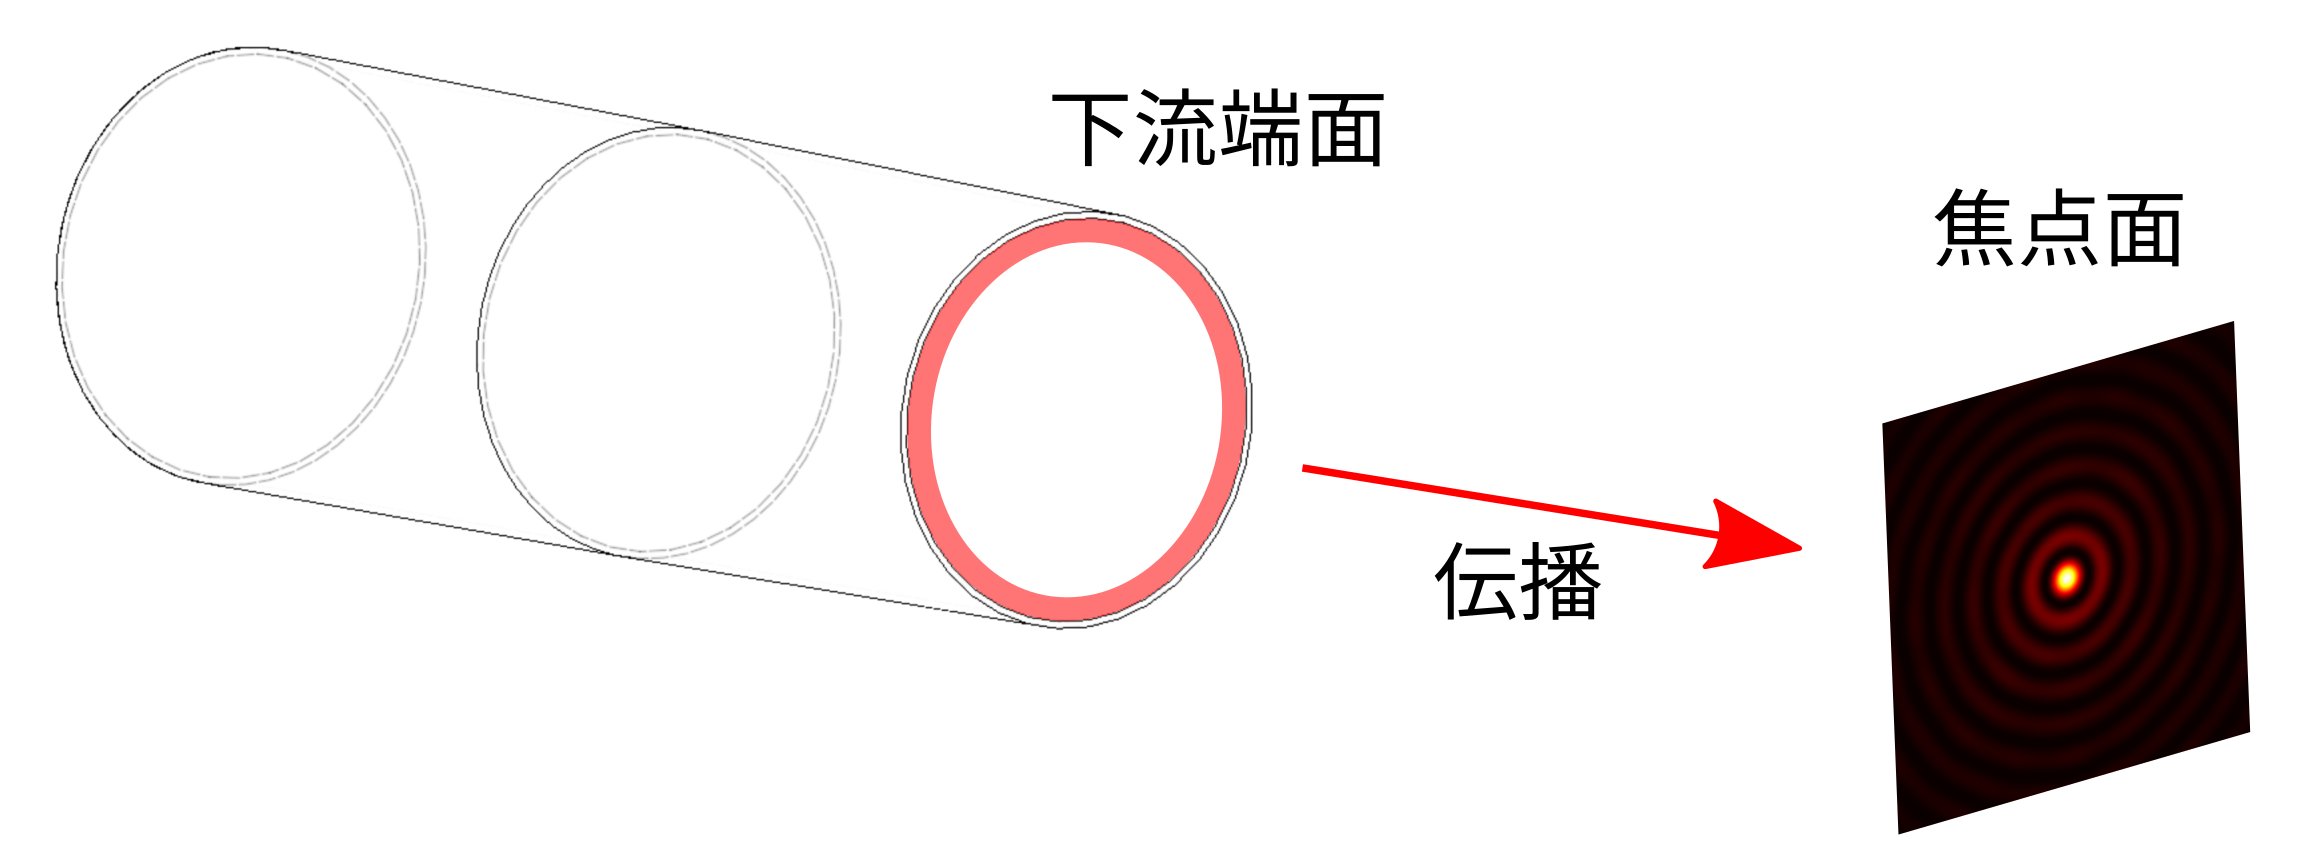
\includegraphics[width=12cm]{method/simulation_schematic.png}
\caption{シミュレーションの概観}
\label{fig:simulation_schematic}
\end{figure}


\begin{figure}[h]
\centering
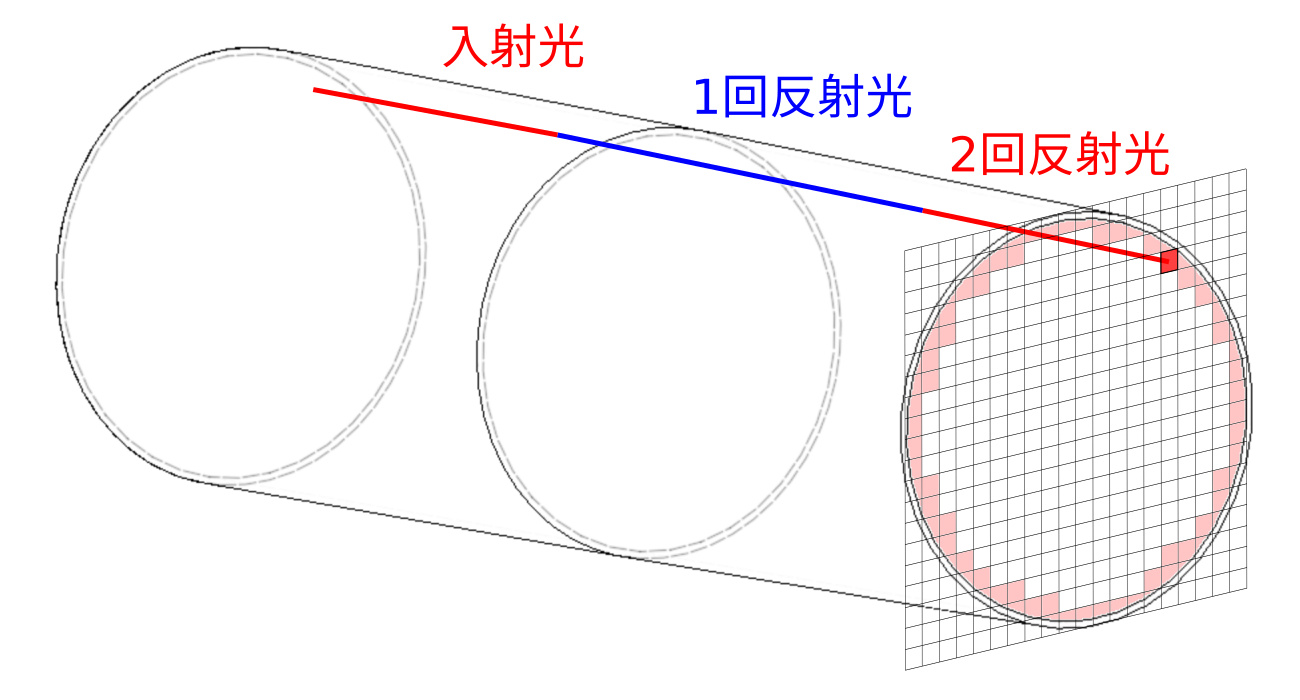
\includegraphics[width=10cm]{method/simulation_raytrace_schematic.png}
\caption{光線追跡による下流端面波動場の計算}
\label{fig:simulation_raytrace}
\end{figure}

\begin{figure}[h]
\centering
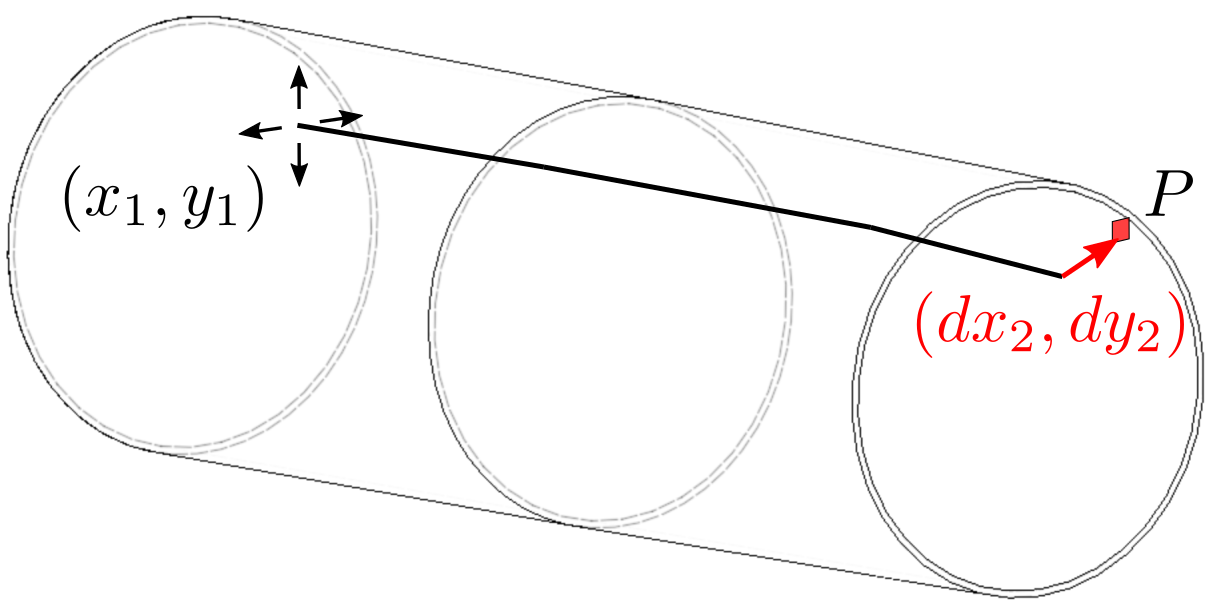
\includegraphics[width=10cm]{method/simulation_backtrace.png}
\caption{点$P$に到達する光路の計算}
\label{fig:simulation_backtrace}
\end{figure}

\begin{figure}[h]
\centering
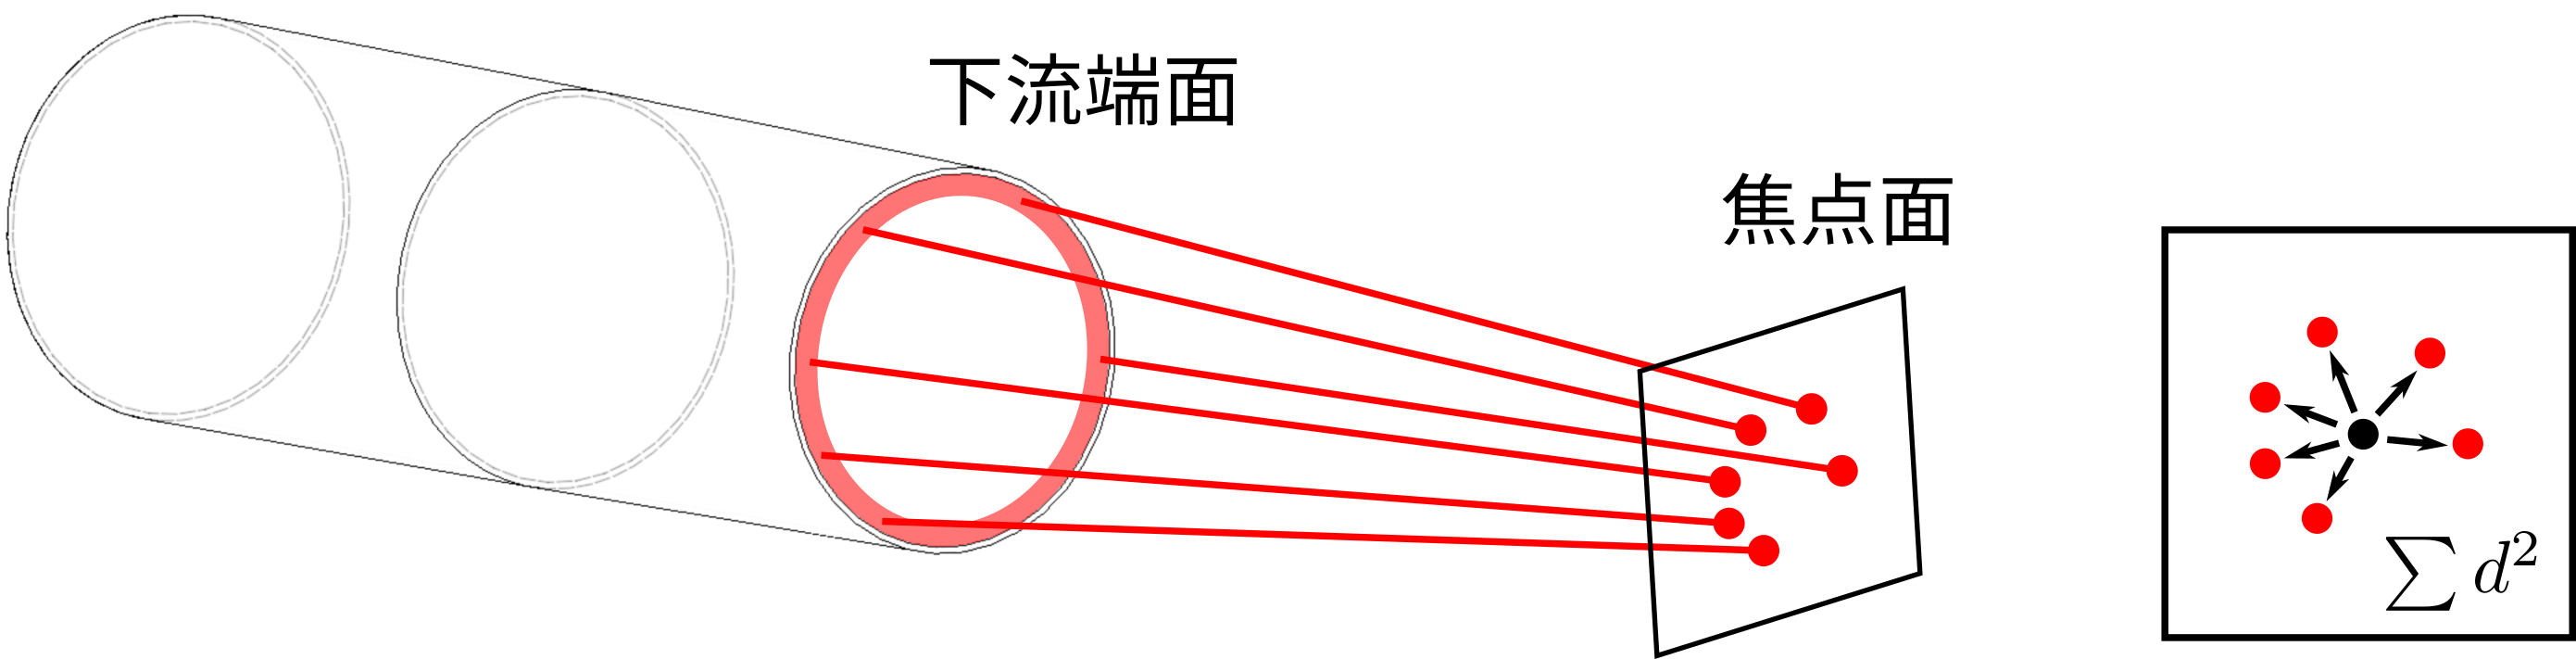
\includegraphics[width=14cm]{method/simulation_focal_point_optimize.png}
\caption{焦点位置の計算}
\label{fig:simulation_focal_point_optimize}
\end{figure}



\clearpage
% ================================================== %
% section
% ================================================== %
\newpage

\section{計算条件}
\label{chap2_simulation_condition}



\subsection{光源の波長・エネルギー}
\label{chap2_incident_beam_energy}

図\ref{fig:corona_spectrum}は、FOXSI3において撮影されたデータから解析された太陽コロナの活動領域におけるX線スペクトルである。\cite{2019AGUFMSH31C3315V}
これをもとに考えれば、測定対象となるX線のエネルギーは数百 eV から 4 keV程度であることになる。

\begin{figure}[ht]
\centering
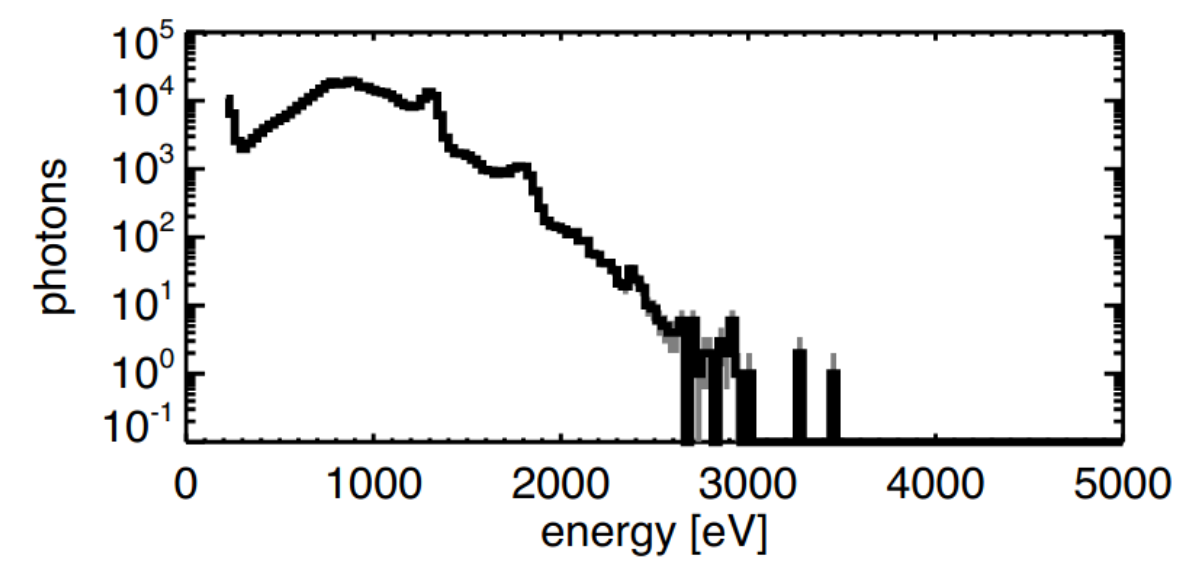
\includegraphics[height=4cm]{corona_spectrum.png}
\caption{太陽コロナ活動領域のX線スペクトル\cite{2019AGUFMSH31C3315V}}
\label{fig:corona_spectrum}
\end{figure}

本章では表\ref{tb:simulation_target_energy}に示すように、厳しい形状精度が求められる 4 keV のX線、および\ref{chap5}章の波面計測実験に用いる可視光ビームの波長 632.8 nm を対象にシミュレーションを行う。

\begin{table}[!ht]
\begin{center}
  \begin{tabular}{|c|c|l|} \hline
    エネルギー & 波長 & 説明 \\ \hline
    4.0 keV & 0.310 nm & 太陽観測時に対称となるX線 \\
    19.59 eV & 632.8 nm & 可視光計測に用いるHe-Neレーザー \\ \hline
  \end{tabular}
  \caption{シミュレーションで入力する波長・エネルギー}
  \label{tb:simulation_target_energy}
\end{center}
\end{table}

\subsection{入力する形状誤差}
\label{chap2_error_input_types}

入力する形状誤差の種類について述べる。

\begin{figure}[!ht]
\centering

\subfloat[直径誤差]{
    
\includegraphics[height=3cm]{error_types/diameter_error_schematic.png}
    \label{fig:diameter_error_schematic}
}
\hspace{5mm}
\subfloat[周方向2山誤差]{
    
\includegraphics[height=3cm]{error_types/oval_error_schematic.png}
    \label{fig:oval_error_schematic}
}
\hspace{5mm}
\subfloat[周方向中周期誤差]{
    
\includegraphics[height=3cm]{error_types/roundness_medium_error_schematic.png}
    \label{fig:roundness_medium_error_schematic}
}
\hspace{5mm}
\subfloat[周方向短周期誤差]{
    
\includegraphics[height=3cm]{error_types/roundness_short_error_schematic.png}
    \label{fig:roundness_short_error_schematic}
}
\\

\subfloat[テーパー角誤差]{
    
\includegraphics[height=3cm]{error_types/taper_error_schematic.png}
    \label{fig:taper_error_schematic}
}
\hspace{5mm}
\subfloat[光軸たわみ]{
    
\includegraphics[height=3cm]{error_types/axis_deflection_schematic.png}
    \label{fig:axis_deflection_schematic}
}
\\

\subfloat[長手方向長周期形状誤差]{
    
\includegraphics[height=3cm]{error_types/profile_long_error_schematic.png}
    \label{fig:profile_long_error_schematic}
}
\hspace{5mm}
\subfloat[長手方向中周期形状誤差]{
    
\includegraphics[height=3cm]{error_types/profile_medium_error_schematic.png}
    \label{fig:profile_medium_error_schematic}
}

\caption[]{入力するミラー形状誤差の種類}
\label{fig:fwhm_explanation}
\end{figure}

\clearpage
% ================================================== %
% section
% ================================================== %
\newpage

\section{理想集光}
\label{chap2_ideal_focusing}

まず、誤差入力を与える前に、誤差のない理想的なミラー形状に対する集光面強度分布を計算し、その特徴について述べる。

\begin{comment}
\begin{figure}[!ht]
\centering

\subfloat[可視光(632.8nm)]{
    \includegraphics[width=3cm]{ideal/visible_light_focus_abs.png}
    \label{fig:visible_light_ideal_focus_abs}
}
\subfloat[300eV]{
    \centering
    \includegraphics[width=3cm]{ideal/300eV_focus_abs.png}
    \label{fig:300eV_ideal_focus_abs}
}
\subfloat[1keV]{
    \centering
    \includegraphics[width=3cm]{ideal/1keV_focus_abs.png}
    \label{fig:1keV_ideal_focus_abs}
}
\subfloat[3keV]{
    \centering
    \includegraphics[width=3cm]{ideal/3keV_focus_abs.png}
    \label{fig:3keV_ideal_focus_abs}
}
\caption[]{理想的なミラーの各波長に対する集光波面}
\label{fig:fwhm_explanation}
\end{figure}
\end{comment}

表\ref{tb:ideal_focus_evaluation}にそれぞれの波長に対するHPDおよびFWHMを示す。
理想集光の場合は集光波面が回転対象になっているため、FWHMは任意の横方向の1本のプロファイルに対してのみ示す。

\begin{table}[!ht]
\begin{center}
  \begin{tabular}{|c|c|c|c|c|} \hline
    項目 & 可視光(632.8nm) & 300eV & 1keV & 3keV \\ \hline
    HPD & 8.989 mm & \SI{23.38}{\micro \metre} & \SI{20.37}{\micro \metre} & \SI{19.45}{\micro \metre} \\
    FWHM & \SI{19.53}{\micro \metre} & \SI{0}{\micro \metre} & \SI{0}{\micro \metre} & \SI{0}{\micro \metre} \\ \hline
  \end{tabular}
  \caption{理想集光の場合のHPDおよびFWHM}
  \label{tb:ideal_focus_evaluation}
\end{center}
\end{table}

\clearpage
% ================================================== %
% section
% ================================================== %
\newpage

\section{各誤差入力に対するシミュレーション}
\label{chap2_simulation_error_response}

本節では、ミラーの製造過程で発生する様々な誤差要因についてその概要を示した上で、それを与えた時の集光波面の変化についてシミュレーションを行う。
シミュレーションでは、\ref{chap2_beam_evaluation_standard}節で述べた3つの評価基準に対応した、許容誤差の閾値を示す。
まず、Strehl比の解析により回折限界集光を達成する上で許容される誤差を評価し、続いて天文用Wolterミラーの達成目標として定めた1秒角分解能の達成に対して求められる許容誤差をHPDおよびFWHMを用いてレイリーの解像限界に照らし合わせて評価する。

\subsection{直径誤差}

\subsection{扁平誤差}

\subsection{周方向形状誤差}

\subsection{長手方向形状誤差}

\subsection{設置角度誤差}

\subsection{設置位置誤差}


\clearpage
% ================================================== %
% section
% ================================================== %
\newpage


\clearpage
% ================================================== %
% section
% ================================================== %
\newpage
\section{収差解析}
\label{chap2_simulation_zernike_analysis}

\ref{chap2_simulation_error_response}節では、ミラー加工において生じる様々な誤差を紹介するとともに、その誤差入力についてのシミュレーションを行った。
本節では、\ref{chap3}章で述べる位相回復によって得られた波面情報から各誤差への分解を行うための解析方法について検討する。

\subsection{Zernike収差}

\subsection{輪帯状の位相分布に対するZernike収差}


\subsection{各誤差に起因する収差の解析}



\section{結言}
\label{chap2_conclusion}



%%%%%%%%%%%%%%%%%%%%%%%%%%%%%%%%%%%%%%%%%%%%%%%%%%%%%%%%%%%%%%%%%%%%%%%%%%%%%
%%% Local Variables:
%%% mode: katex
%%% TeX-master: "../thesis"
%%% End:
